\section{Результаты}

С применением перекрестной проверки была проведена оценка точности классификаторов, обученных на трех различных 
наборах данных с наборами подобранных разными алгоритмами параметрами, а также с параметрами по умолчанию.

Полученные оценки изображены на диаграмме — Рисунок \ref{CrossValAcc}. 
Полученные в результате выполнения программы измерения точности приведены в Таблице \ref{table2}. 

\begin{figure}[H]
    \centering
    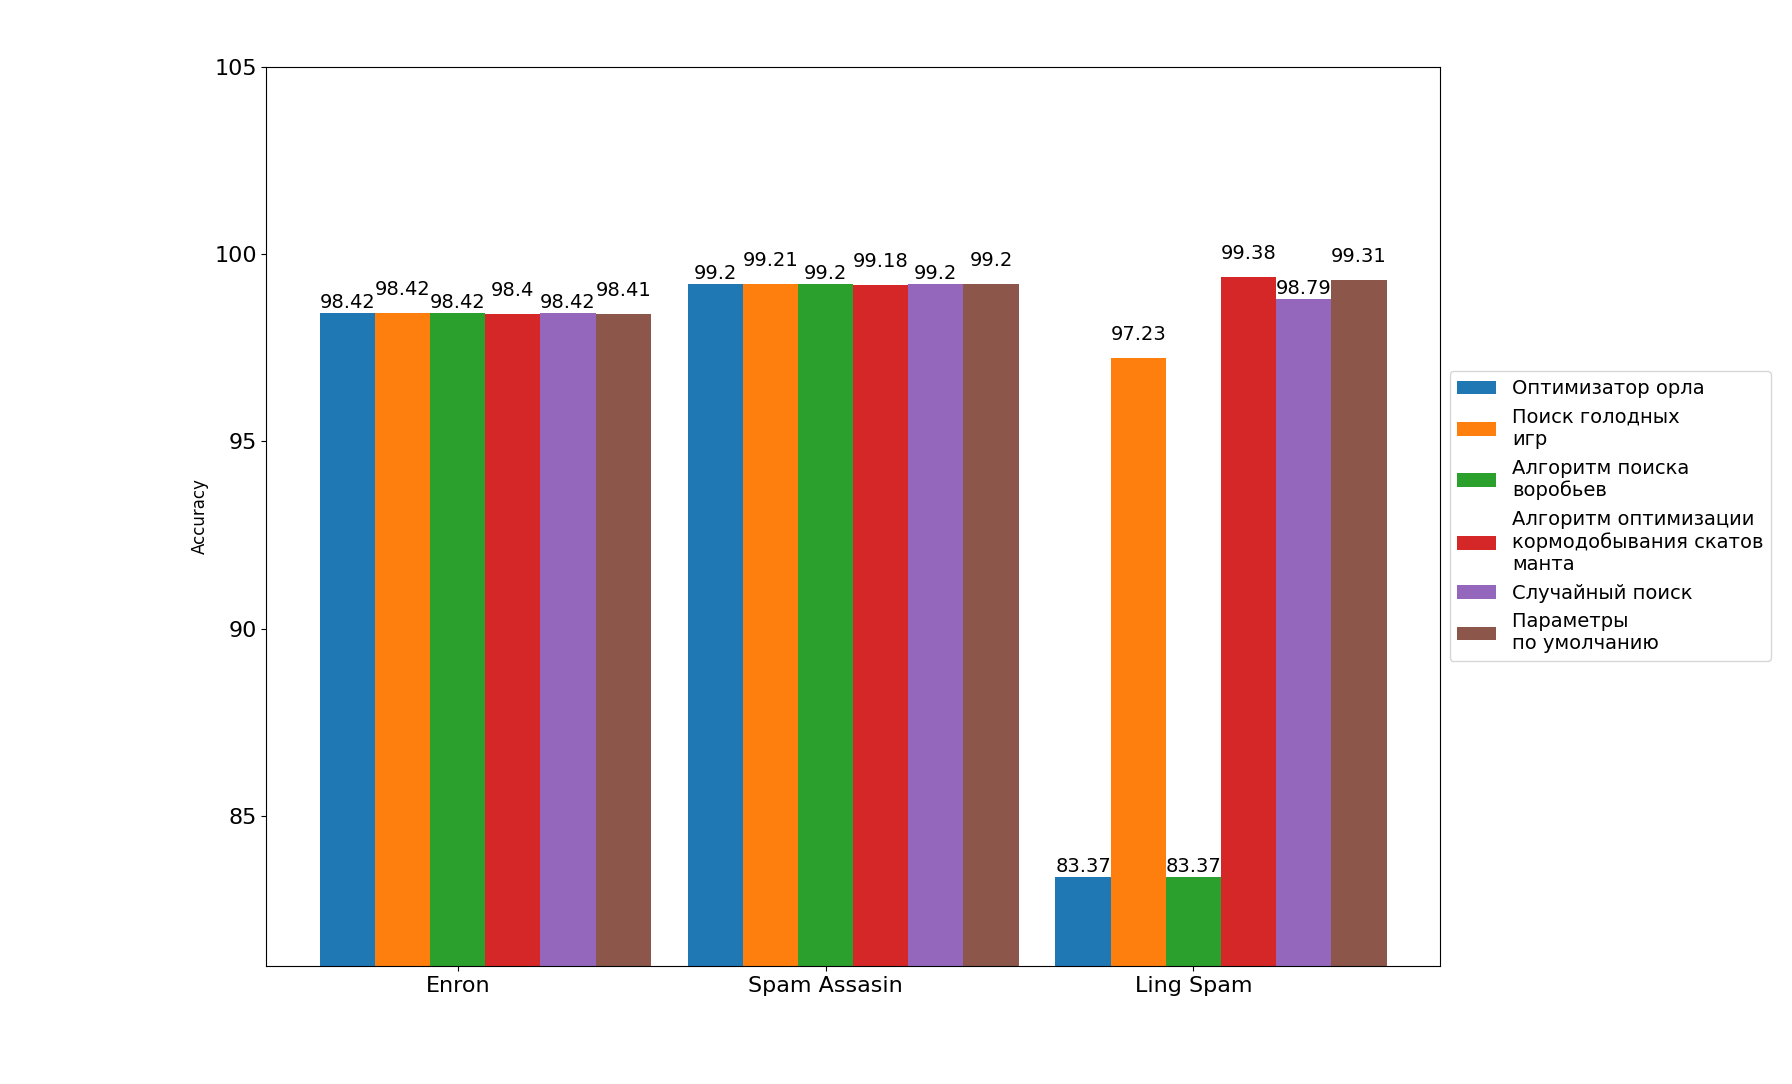
\includegraphics[width=165mm]{static/cross-val-acc.png}
    \caption{Точность для возможных сочетаний наборов данных и алгоритмов оптимизации}
    \label{CrossValAcc}
\end{figure}

Затем обученные на одних данных классификаторы были применены к данным, не применявшихся при обучении. Также была 
измерена точность. Результаты измерений занесены в Таблицу \ref{table2}.
\\
\\
\\
\\
\begin{table}[]
    \centering
    \caption{Результаты эксперимента — метрика "Точность"}
    \begin{tabular}{|c|l|c|c|c|c|c|c|}
    \hline
    \multicolumn{1}{|l|}{\begin{tabular}[c]{@{}l@{}}Обучающие \\ данные\end{tabular}} & Данные & \multicolumn{1}{l|}{MRFO} & \multicolumn{1}{l|}{HGS} & \multicolumn{1}{l|}{AO} & \multicolumn{1}{l|}{SSA} & \multicolumn{1}{l|}{RSCV} & \multicolumn{1}{l|}{DEFAULT} \\ \hline
    \multirow{2}{*}{LS}                                                               & SA     & 90.217                    & 89.480                   & 75.287                  & 75.287                   & 88.082                    & 88.711                       \\ \cline{2-8} 
                                                                                      & EN     & 70.675                    & 76.482                   & 50.927                  & 50.915                   & 76.183                    & 70.343                       \\ \hline
    \multirow{2}{*}{SA}                                                               & LS     & 94.988                    & 95.092                   & 95.022                  & 95.299                   & 94.469                    & 94.469                       \\ \cline{2-8} 
                                                                                      & EN     & 72.852                    & 74.901                   & 74.901                  & 73.086                   & 74.587                    & 73.768                       \\ \hline
    \multirow{2}{*}{EN}                                                               & LS     & 90.840                    & 91.116                   & 89.803                  & 89.803                   & 89.803                    & 81.645                       \\ \cline{2-8} 
                                                                                      & SA     & 87.606                    & 86.696                   & 86.457                  & 86.457                   & 86.457                    & 77.356                       \\ \hline
    \end{tabular}
    \label{table2}
\end{table}

Также по результатам применения полученных классификаторов к новым данным построены кривые ошибок, с указанием 
площади под ней. На Рисунке \ref{EN-LS} изображена кривая ошибок для классификатора, обученного на наборе Enron и 
примененного к набору Ling Spam, на Рисунке \ref{EN-SA} — для обученного на Enron и примененного к Spam Assasin, и 
так далее.

\begin{figure}[H]
    \centering
    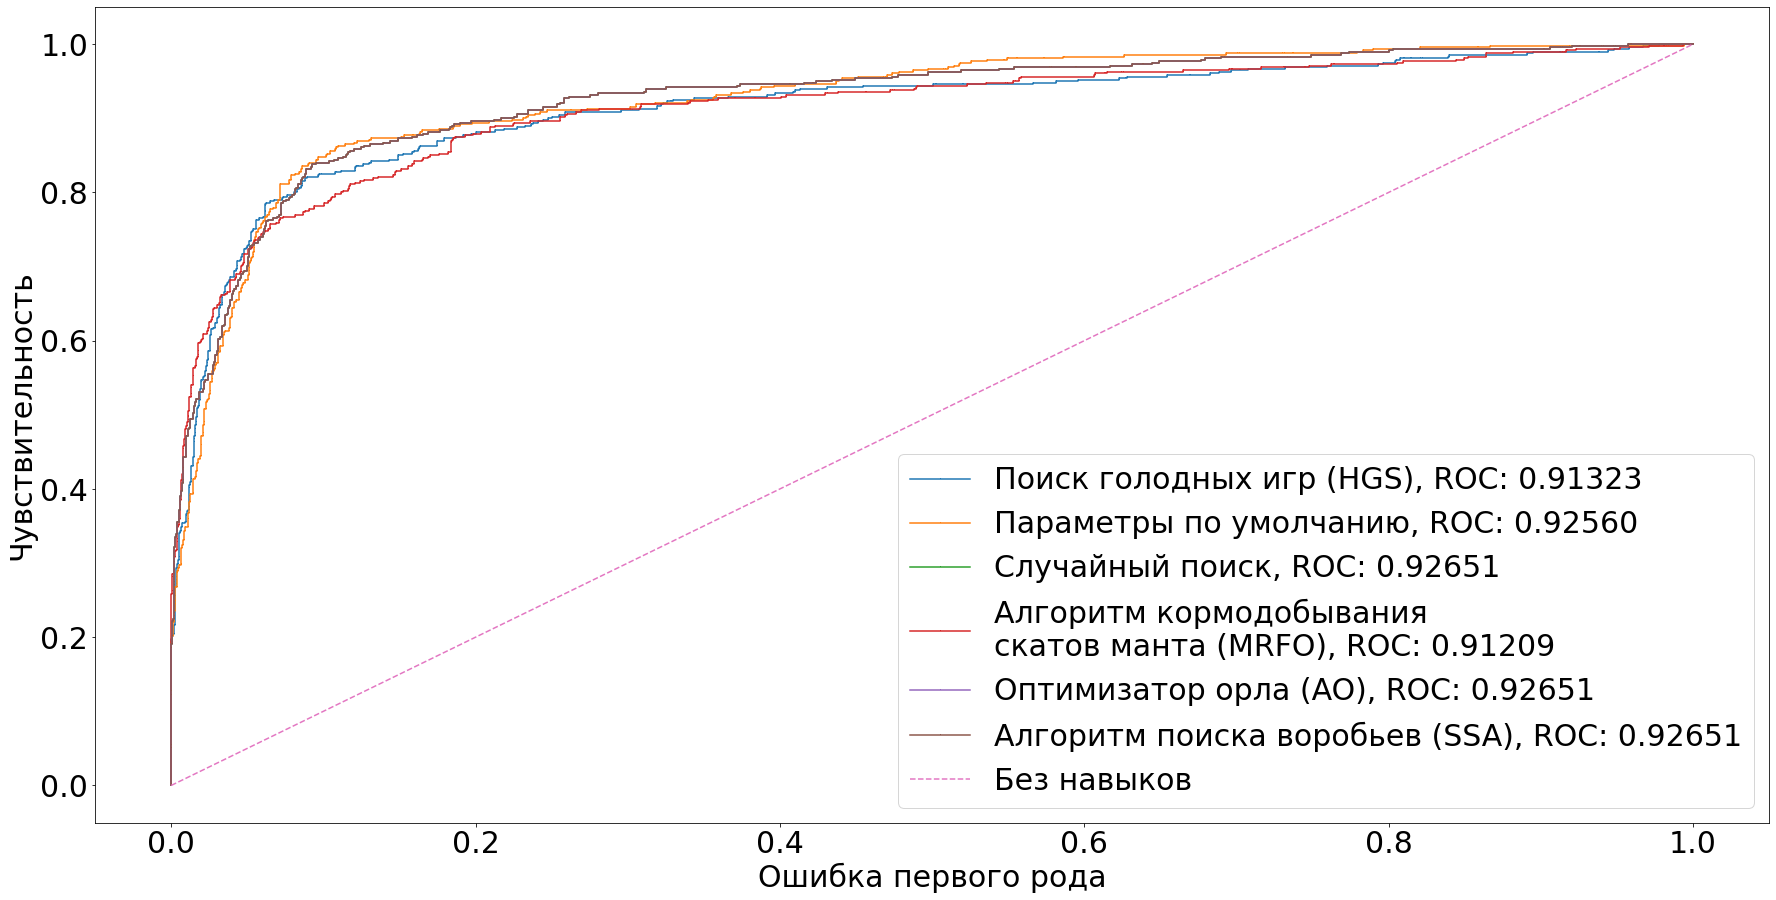
\includegraphics[width=165mm]{static/EN-LS.png}
    \caption{Кривые ошибок для классификаторов, обученных на Enron, оцененных — на Ling Spam}
    \label{EN-LS}
\end{figure}

\begin{figure}[H]
    \centering
    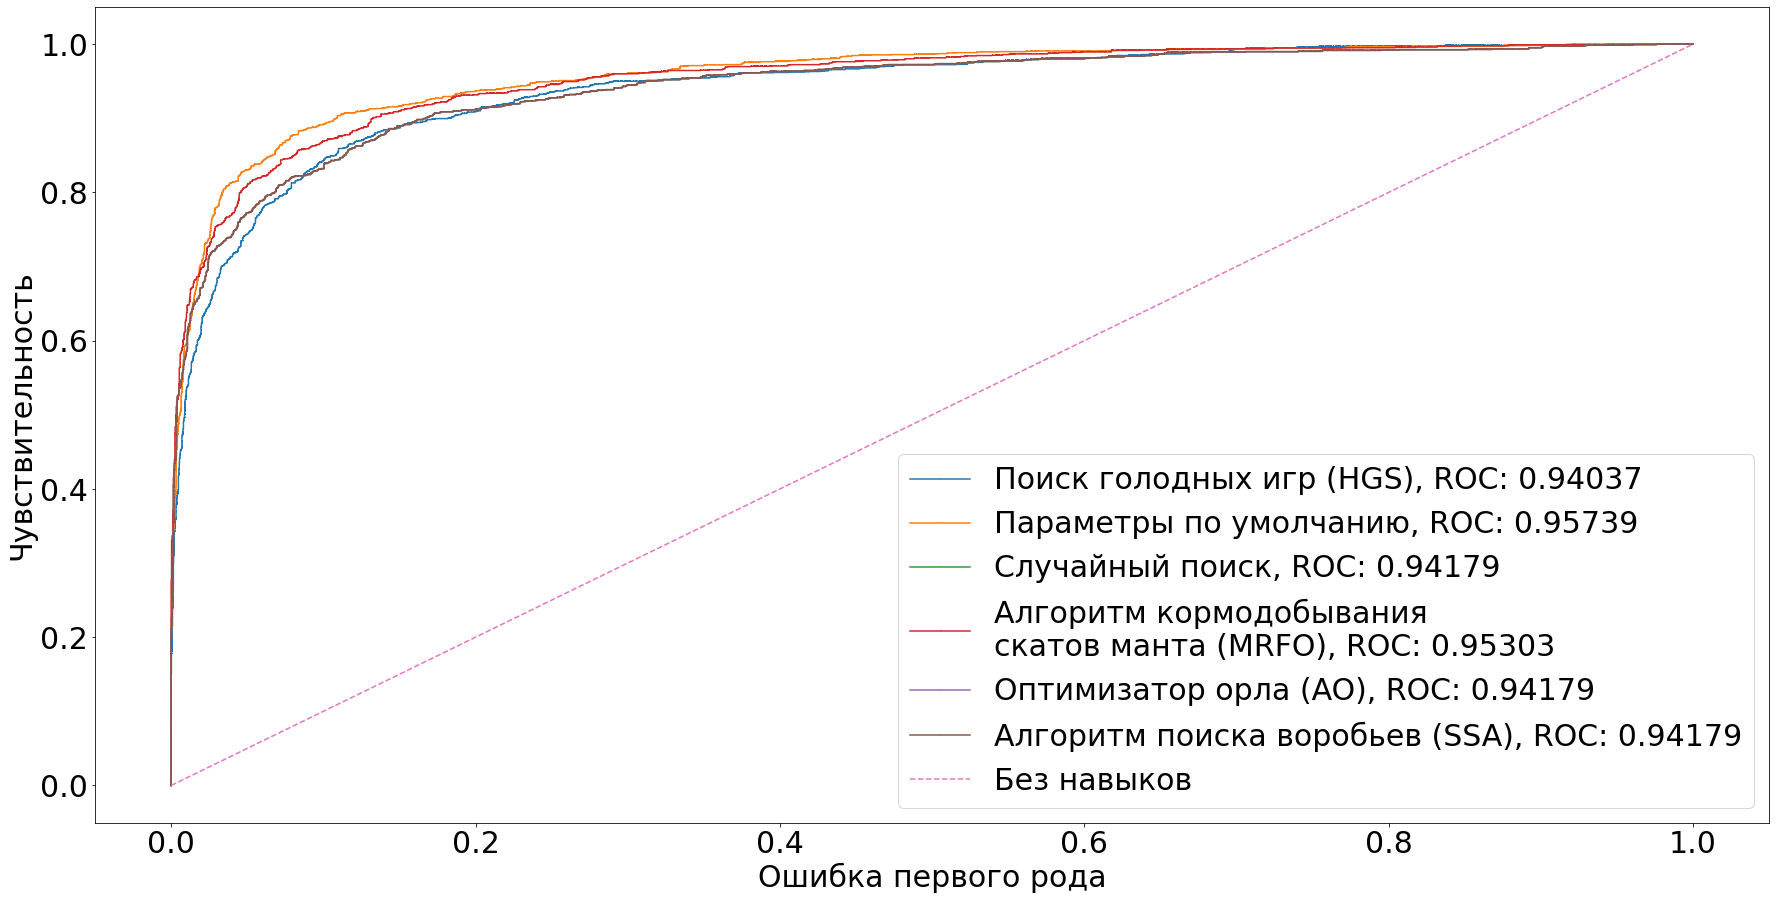
\includegraphics[width=165mm]{static/EN-SA.png}
    \caption{Кривые ошибок для классификаторов, обученных на Enron, оцененных — на Spam Assasin}
    \label{EN-SA}
\end{figure}

На следующих рисунках — Рисунке \ref{SA-LS}, Рисунке \ref{SA-EN}, Рисунке \ref{LS-SA} и Рисунке \ref{LS-EN} — 
изображены кривые, соответствующие наборам данных, указанным в названиях рисунков.

\begin{figure}[H]
    \centering
    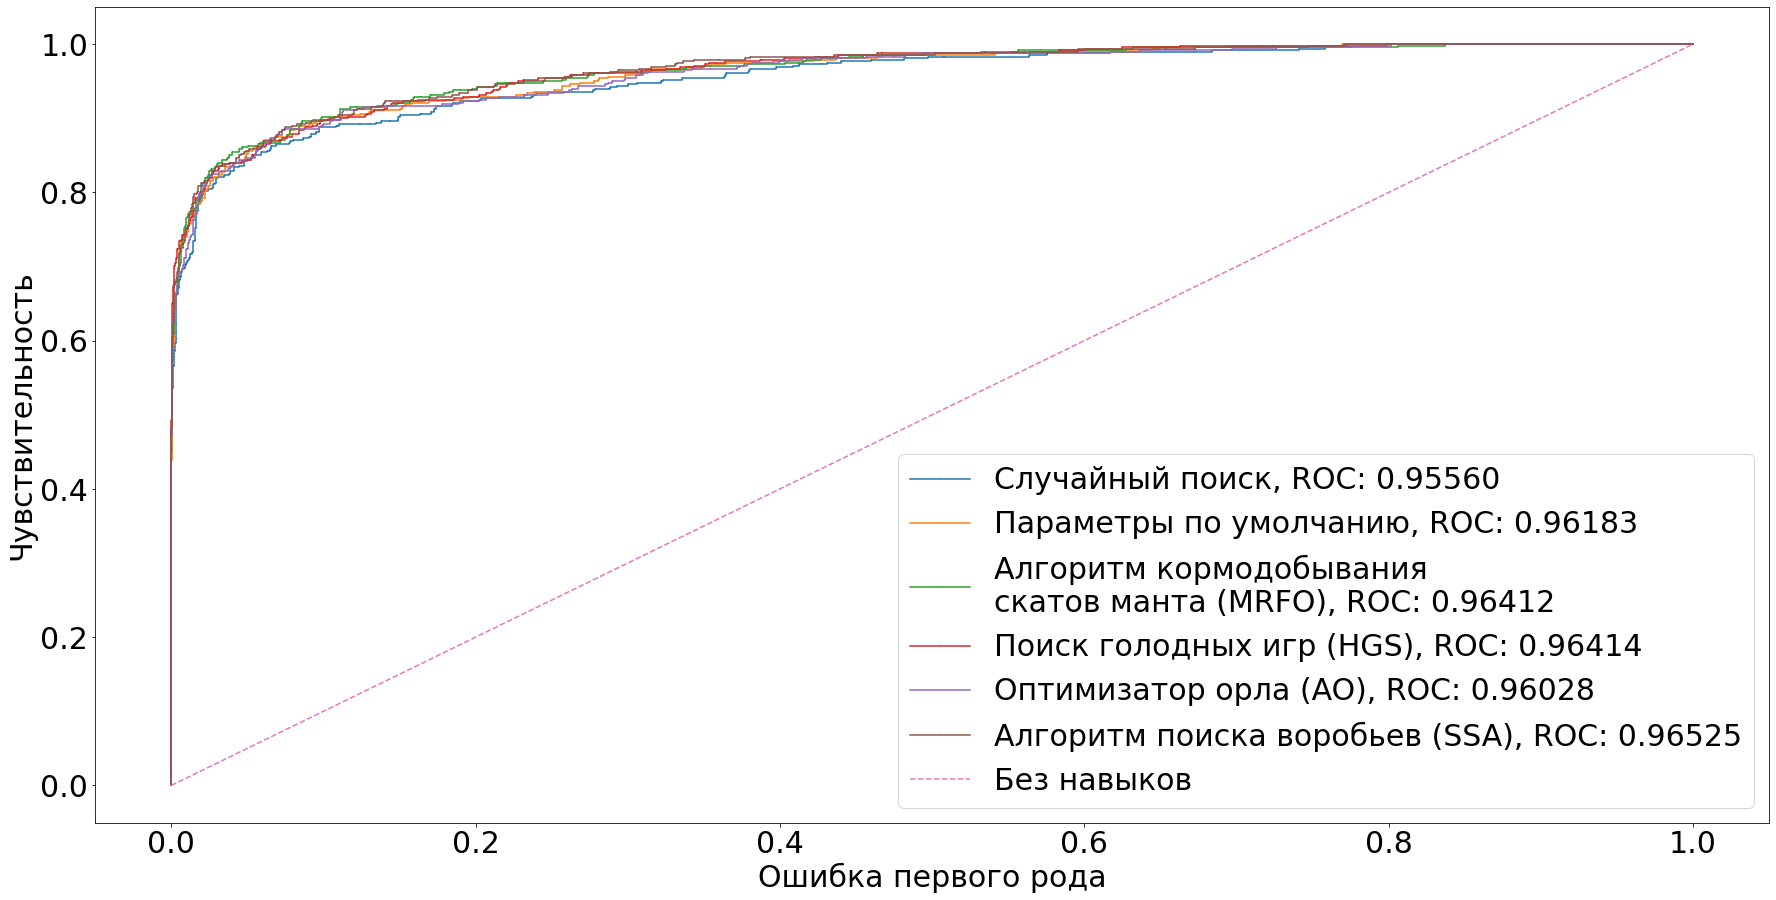
\includegraphics[width=165mm]{static/SA-LS.png}
    \caption{Кривые ошибок для классификаторов, обученных на Spam Assasin, оцененных — на Ling Spam}
    \label{SA-LS}
\end{figure}

\begin{figure}[H]
    \centering
    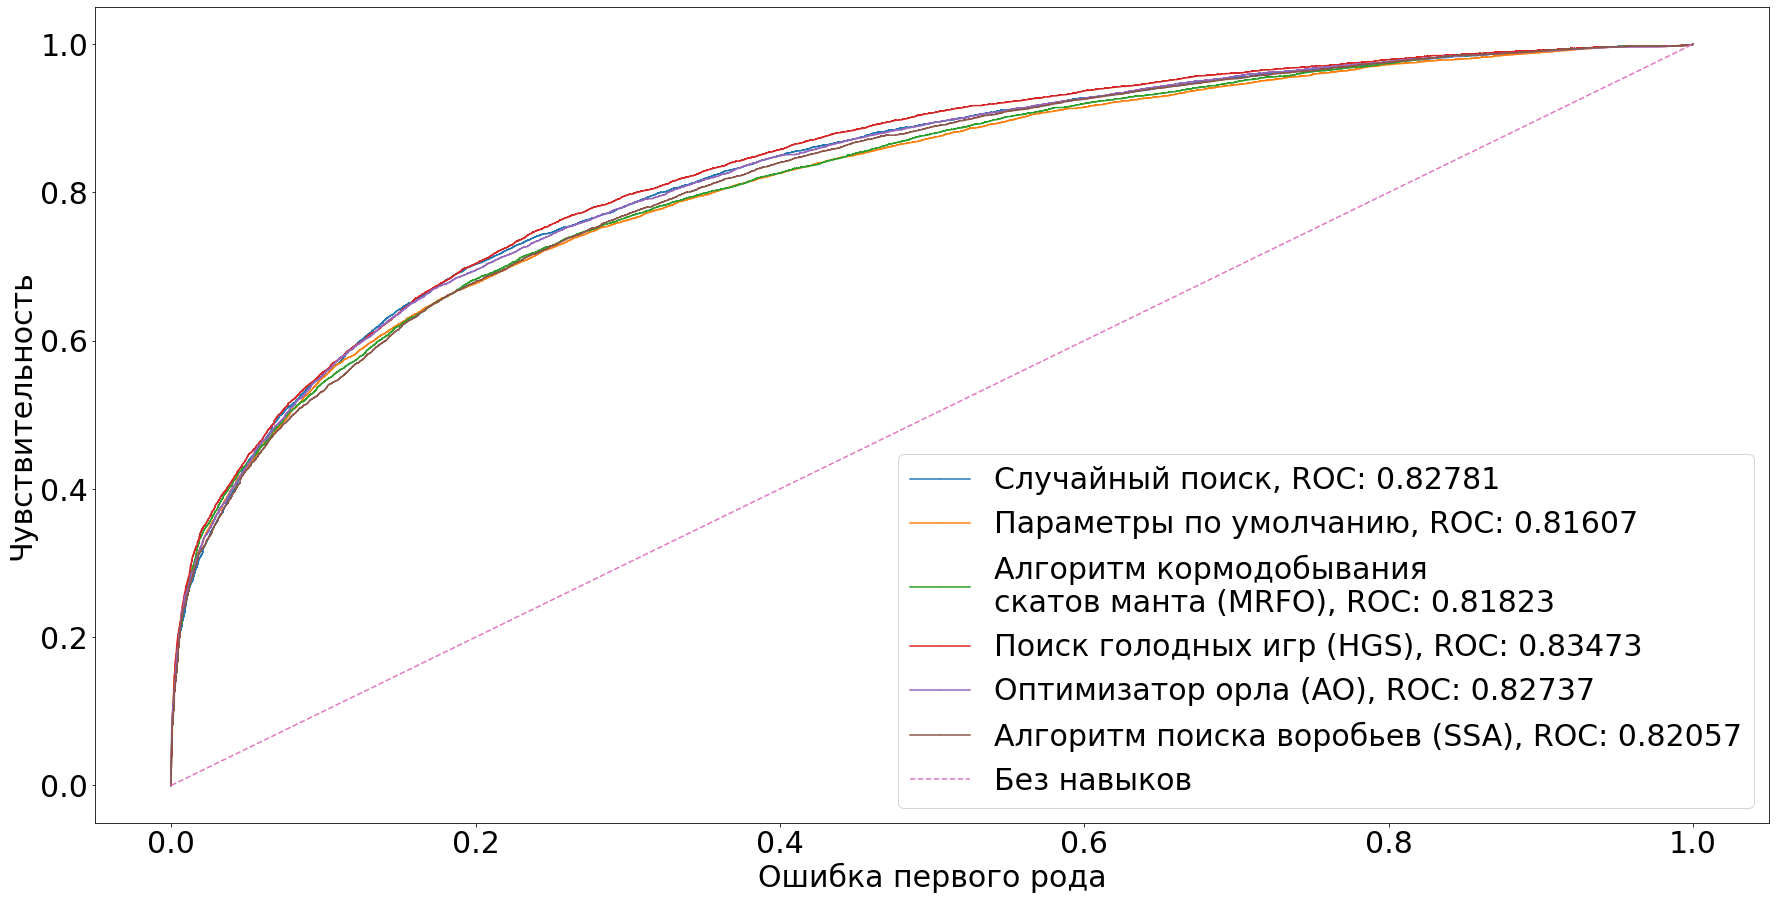
\includegraphics[width=165mm]{static/SA-EN.png}
    \caption{Кривые ошибок для классификаторов, обученных на Spam Assasin, оцененных — на Enron}
    \label{SA-EN}
\end{figure}

\begin{figure}[H]
    \centering
    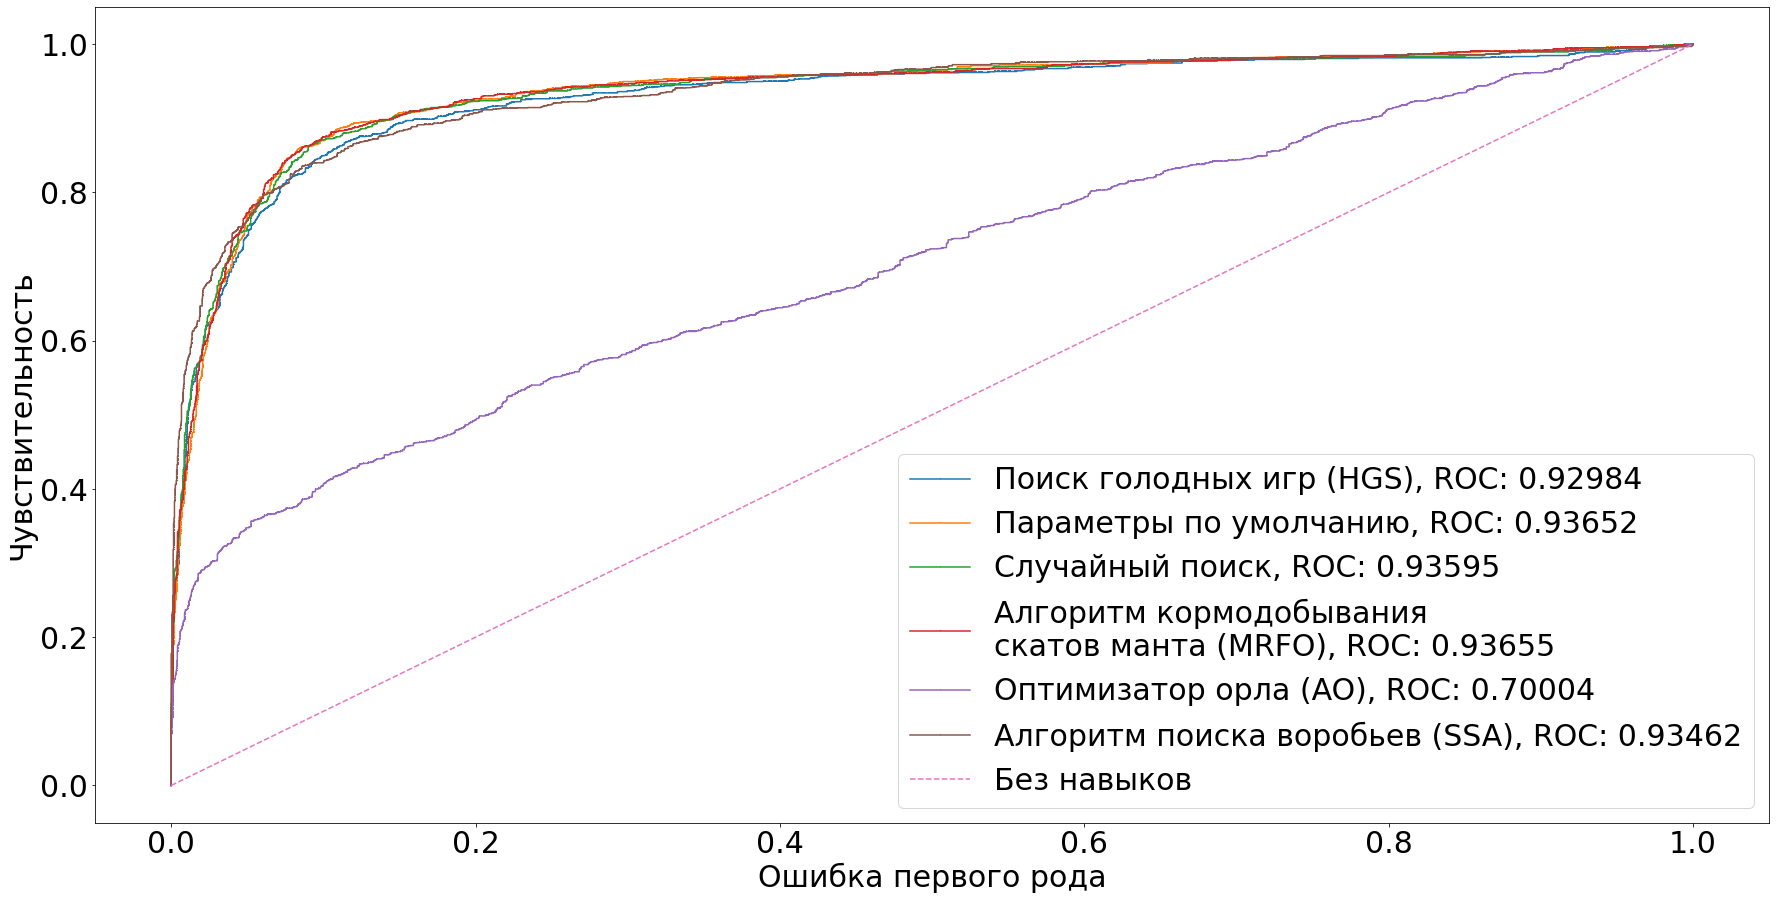
\includegraphics[width=165mm]{static/LS-SA.png}
    \caption{Кривые ошибок для классификаторов, обученных на Ling Spam, оцененных — на Spam Assasin}
    \label{LS-SA}
\end{figure}

\begin{figure}[H]
    \centering
    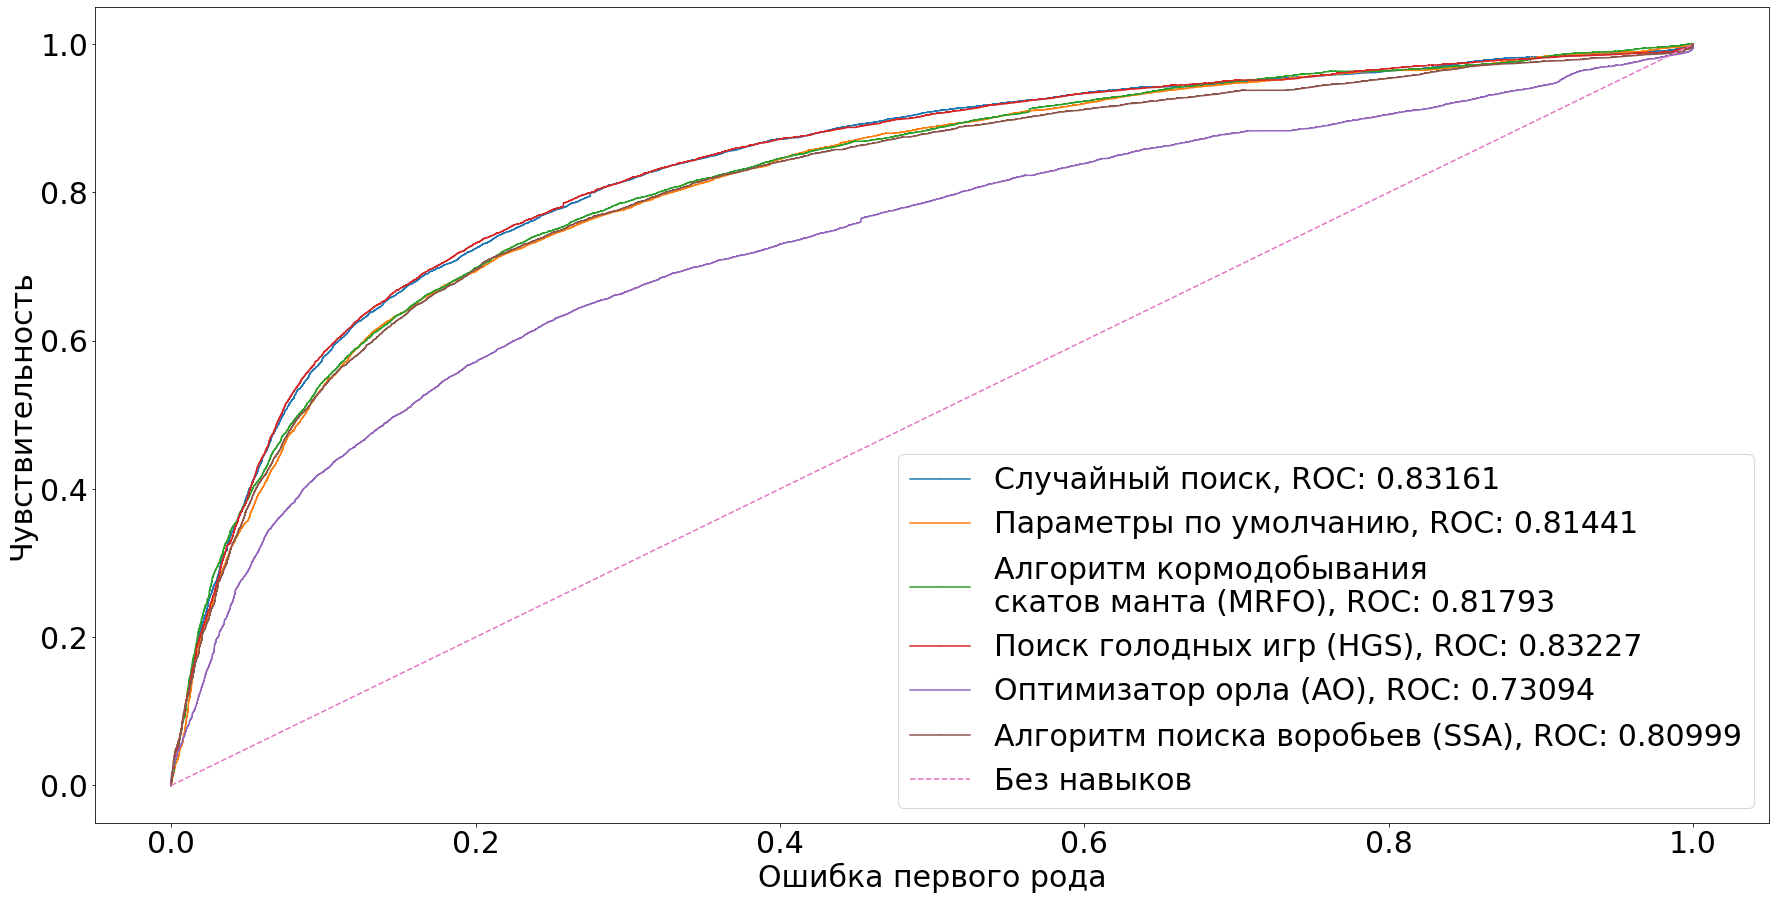
\includegraphics[width=165mm]{static/LS-EN.png}
    \caption{Кривые ошибок для классификаторов, обученных на Ling Spam, оцененных — на Enron}
    \label{LS-EN}
\end{figure}

Анализируя результаты, можно сделать следующие выводы:

\begin{itemize}
    \item[—] Алгоритм MRFO по метрике точность на новых данных превзошел параметры по умолчанию в 5 из 6 случаев,
    случайный поиск — в 4 из 6, при чем в 2 из этих 4 случаев стал лучшим по сравнению с другими природными алгоритмами.
    Однако по площади под кривой — только в 2 из 6 случаев алгоритм превзошел случайный поиск и параметры по умолчанию.  
    Лучшим стал 1 раз из этих 2;
    
    \item[—] Алгоритм HGS по метрике точность на новых данных превзошел как параметры по умолчанию, так и 
    случайный поиск во всех 6 случаях, являлся лучшим в 3 из 6 случаях.
    По площади под кривой — трижды превзошел случайный поиск и параметры по умолчанию, дважды дал лучшие показатели;

    \item[—] Алгоритмы SSA и AO, хоть и показали на новых данных в большинстве случаев 
    более высокую точность по сравнению со случайным поиском и параметрами по умолчанию, по показателю площади 
    под кривой ошибок $ROC$ оказались значительно хуже других алгоритмов;

    \item[—] Влияние настройки параметров на эффективность алгоритмов более заметно на меньших объемах данных. 
    По результатам в Таблице \ref{table2} видно, что при использовании для обучения большого набора данных Enron, 
    алгоритмы оптимизации в большинстве случаев дают такое же улучшение, как и случайный поиск;
    
    \item[—] "Поиск голодных игр" (HGS) позволил улучшить производительность по обеим метрикам чаще других выбранных  
    алгоритмов.
\end{itemize}
